\chapter{Os espaços \texorpdfstring{$\mathbb R^n$}{Rn}}

Neste capítulo, introduziremos os espaços $\mathbb R^n$, que generalizam a reta real $\mathbb R$ para pontos com um número finito de coordenadas, bem como algumas de suas operações mais básicas.

Para cada inteiro $n\geq 1$, o espaço $\mathbb R^n$ é o conjunto das $n$-tuplas ordenadas de números reais. Assim, seus elementos são pontos da forma
\[
    p=(x_1,\dots,x_n),
\]
com $x_i\in\mathbb R$ para cada $i=1,\dots,n$.

\section{Introdução}\index{espaço euclidiano}
Um ponto $p \in \mathbb R^n$ é descrito por $n$ coordenadas reais.
\[
    p = (x_1, \dots, x_n).
\]

Lembremos que $\mathbb R^2$ é o conjunto de todos os pares ordenados $(x, y)$, onde $x, y \in \mathbb R$.
Em símbolos:
\begin{equation*}
    \mathbb R^2 = \{(x, y) : x, y \in \mathbb R\}.
\end{equation*}

Em analogia à representação de $\mathbb R$ como uma reta, podemos visualizar $\mathbb R^2$ como o conjunto dos pontos de um plano cartesiano.

Na Figura~\ref{fig:plano-cartesiano}, o ponto $(2,3)$ está posicionado $2$ unidades no sentido positivo do eixo $x$ e $3$ unidades no sentido positivo do eixo $y$.

\begin{figure}[ht]
    \centering
    \begin{tikzpicture}
    \draw[->,ultra thick] (-4,0)--(4,0) node[right]{$x$};
    \draw[->,ultra thick] (0,-4)--(0,4) node[above]{$y$};
    % Ponto (2,3)
    \filldraw[black] (2,3) circle (2pt);
    \node[above right] at (2,3) {$(2,3)$};
    \draw[dotted] (2,0) -- (2,3);
    \draw[dotted] (0,3) -- (2,3);
    \draw (2,0.1) -- (2,-0.1);
    \node[below] at (2,0) {2};
    \draw (0.1,3) -- (-0.1,3);
    \node[left] at (0,3) {3};
    \node[below left] at (0,0) {0};

    \end{tikzpicture}
    \caption{O plano cartesiano.}
    \label{fig:plano-cartesiano}
\end{figure}

Por sua vez, o conjunto de todas as triplas ordenadas de números reais é denotado por $\mathbb R^3$.
Em símbolos:
\begin{equation*}
    \mathbb R^3 = \{(x, y, z) : x, y, z \in \mathbb R\}.
\end{equation*}

Seguindo o padrão já comentado, podemos visualizar $\mathbb R^3$ como o conjunto dos pontos do espaço tridimensional.

A tripla $(x,y,z)$ representa um ponto com três coordenadas: a primeira associada ao eixo $x$, a segunda ao eixo $y$ e a terceira ao eixo $z$.
O ponto $(2,3,1)$ está representado na Figura~\ref{fig:espaco-tridimensional}.

\begin{figure}[ht]
    \centering
    \tdplotsetmaincoords{70}{110}
    \begin{tikzpicture}[tdplot_main_coords]
    % Eixos
    \draw[->,ultra thick] (-4,0,0)--(4,0,0) node[right]{$x$};
    \draw[->,ultra thick] (0,-4,0)--(0,4,0) node[above]{$y$};
    \draw[->,ultra thick] (0,0,-4)--(0,0,4) node[above]{$z$};
    % Ponto (2,3,1)
    \filldraw[black] (2,3,1) circle (2pt);
    \node[above right] at (2,3,1) {$(2,3,1)$};
    % Linhas pontilhadas
    \draw[dotted] (2,0,0) -- (2,3,0) -- (2,3,1);
    \draw[dotted] (0,3,0) -- (2,3,0);
    \draw[dotted] (2,0,0) -- (2,0,1) -- (2,3,1);
    \draw[dotted] (0,0,1) -- (2,0,1);
    % Marcas nos eixos
    \draw (2,0.1,0) -- (2,-0.1,0);
    \node[below] at (2,0,0) {2};
    \draw (0.1,3,0) -- (-0.1,3,0);
    \node[left] at (0,3,0) {3};
    \draw (0.1,0,1) -- (-0.1,0,1);
    \node[left] at (0,0,1) {1};
    \node[below left] at (0,0,0) {0};

    \end{tikzpicture}
    \caption{O espaço tridimensional.}
    \label{fig:espaco-tridimensional}
\end{figure}

De modo geral, para cada inteiro $n\geq 1$, o conjunto $\mathbb R^n$ é o conjunto de todas as $n$-tuplas ordenadas de números reais:
\begin{equation*}
    \mathbb R^n = \{(x_1, \ldots, x_n) : x_1, \ldots, x_n \in \mathbb R\}.
\end{equation*}

Para $n\geq 4$, esse conjunto não possui uma representação gráfica simples no estilo dos casos anteriores, de dimensões menores.
Porém, a teoria desenvolvida para $\mathbb R^n$, com $n\geq 4$, é uma extensão natural da teoria desenvolvida para $\mathbb R$, $\mathbb R^2$ e $\mathbb R^3$, e possui amplas aplicações práticas e teóricas.

Cada espaço $\mathbb R^n$ possui um elemento denominado \emph{origem}\index{origem}, denotado por $\vec 0$, ou simplesmente por $0$, cujas coordenadas são todas iguais ao número real $0$.
\begin{equation*}
    \vec 0 = (0, \ldots, 0).
\end{equation*}

Um detalhe que pode ser confuso à primeira vista, mas que não gera confusão, na prática, é que a notação $0$ é utilizada tanto para o número real $0$ quanto para a origem $\vec 0$ de $\mathbb R^n$.
Ao se escrever $0=(0, \ldots, 0)$, o primeiro símbolo $0$ representa a origem de $\mathbb R^n$, enquanto os demais representam o número real $0$, sendo, portanto, objetos de natureza diferente.

No caso $n=1$, identificamos usualmente a $1$-tupla $(x)$ com o próprio número real $x$, de modo que $\mathbb R^1$ é identificado com $\mathbb R$.
Com essa identificação, a origem de $\mathbb R^1$ é o número real $0$.

Elementos de $\mathbb R^n$ serão frequentemente chamados de \emph{pontos}\index{ponto} ou \emph{vetores}\index{vetor}.
Essa dupla nomenclatura reflete duas formas diferentes de interpretar o mesmo objeto matemático.
A palavra \emph{ponto} será usualmente utilizada em situações em que se faz referência a posições no espaço, enquanto a palavra \emph{vetor} é mais utilizada em situações em que pensamos no segmento orientado que parte da origem $\vec 0=(0, \ldots, 0)$\index{origem} e termina no ponto em questão.
Quando esse ponto não é a origem, esse segmento determina, intuitivamente, uma direção, um sentido e um comprimento.
Quando esse ponto é a origem, obtemos o \emph{vetor nulo}\index{vetor nulo}, que possui comprimento zero e não determina uma direção ou um sentido.

O conjunto $\mathbb R^n$, munido das operações e da distância usuais que estudaremos a seguir, é chamado de \emph{espaço euclidiano} $n$-dimensional.
\section{Operações em \texorpdfstring{$\mathbb R^n$}{Rn}}

Algumas operações importantes em $\mathbb R^n$ incluem soma, produto por escalar e produto escalar.
Nesta seção, revisaremos tais operações.

\begin{definition}
    Sejam $p=(x_1, \ldots, x_n)$ e $q=(y_1, \ldots, y_n)$ dois elementos de $\mathbb R^n$, e $\alpha \in \mathbb R$ um número real.
    A \emph{soma}\index{soma vetorial} $p+q$ é definida como:
    \begin{equation*}
        p+q =(x_1, \ldots, x_n)+(y_1, \ldots, y_n)=(x_1+y_1, \ldots, x_n+y_n).
    \end{equation*}
    A \emph{multiplicação por escalar}\index{multiplicação por escalar} $\alpha p$ é definida como:
    \begin{equation*}
        \alpha p = \alpha (x_1, \ldots, x_n) = (\alpha x_1, \ldots, \alpha x_n).
    \end{equation*}
    O \emph{produto escalar}\index{produto escalar} $p \cdot q$ é definido como:
    \begin{equation*}
        p \cdot q = (x_1, \ldots, x_n) \cdot (y_1, \ldots, y_n) = x_1y_1 + \ldots + x_ny_n=\sum_{i=1}^n x_iy_i.
    \end{equation*}
\end{definition}

Como usual, escrevemos
\[
    -p=(-1)p
    \quad\text{e}\quad
    p-q=p+(-q).
\]

Desse modo, $-(x_1, \ldots, x_n) = (-x_1, \ldots, -x_n)$ e $(x_1, \ldots, x_n)-(y_1, \ldots, y_n) = (x_1-y_1, \ldots, x_n-y_n)$.

Note que $p+q$ e $\alpha p$ são elementos de $\mathbb R^n$, enquanto $p\cdot q$ é um número real.
Assim, a soma e a multiplicação por escalar produzem vetores, ao passo que o produto escalar associa dois vetores a um escalar.

\begin{example}
    Se $p=(1,-2,3)$, $q=(4,0,-1)$ e $\alpha=-2$, então:
    \[
        p+q=(5,-2,2),
        \qquad
        \alpha p=(-2,4,-6),
    \]
    e
    \[
        p\cdot q
        =1\cdot4+(-2)\cdot0+3\cdot(-1)
        =1.
    \]
\end{example}

\begin{example}
    Se $p=(3,-1,2)$ e $q=(1,4,-2)$, então
    \[
        q-p=(1,4,-2)-(3,-1,2)=(-2,5,-4).
    \]
    Assim, partindo de $p$ e somando o deslocamento $q-p$, chegamos a $q$:
    \[
        p+(q-p)
        =(3,-1,2)+(-2,5,-4)
        =(1,4,-2)
        =q.
    \]
\end{example}

Vamos lembrar de importantes interpretações geométricas da soma e da multiplicação por escalar.

A soma dos vetores $v=(3, 2)$ e $w=(-1, 1)$ pode ser visualizada como o vetor com início na origem e fim no ponto obtido posicionando-se o vetor $w$ com início no ponto final do vetor $v$, conforme ilustrado na Figura~\ref{fig:soma-vetores}.

\subimport{operacoesRn}{somaVetores}
A multiplicação do vetor $v=(1, 2)$ por $2$ e por $-2$ corresponde, respectivamente, a multiplicar o comprimento de $v$ por $2$, mantendo a direção e o sentido, e a multiplicar o comprimento de $v$ por $2$, mantendo a direção e invertendo o sentido, conforme ilustrado na Figura~\ref{fig:produto-por-escalar}.

\subimport{operacoesRn}{produtoPorEscalar}

\begin{example}
    Seja $v=(2,-1)$. Então
    \[
        0v=(0,0),
        \qquad
        \frac12v=(1,-\tfrac12),
        \qquad
        -3v=(-6,3).
    \]
    Multiplicar um vetor por $0$ resulta no vetor nulo.
    
    Multiplicar um vetor por $\frac12$ preserva a direção e o sentido, mas reduz o comprimento pela metade.
    
    Já multiplicar um vetor por $-3$ preserva a direção, inverte o sentido e multiplica o comprimento por $3$.
\end{example}

Agora vamos nos voltar ao produto escalar.

\begin{example}
    O produto escalar entre dois vetores pode ser positivo, nulo ou negativo.
    Por exemplo, tomando $u=(1,2)$, temos:
    \[
        u\cdot(2,1)=1\cdot2+2\cdot1=4>0,
    \]
    \[
        u\cdot(2,-1)=1\cdot2+2\cdot(-1)=0,
    \]
    e
    \[
        u\cdot(-1,-2)=1\cdot(-1)+2\cdot(-2)=-5<0.
    \]
    Por outro lado,
    \[
        u\cdot u=1^2+2^2=5>0.
    \]
\end{example}

Algumas propriedades importantes do produto escalar são as seguintes.

\begin{proposition}\index{produto escalar!propriedades}
    Sejam $p, q, r \in \mathbb R^n$ e $\alpha \in \mathbb R$. Então:
    \begin{enumerate}
        \item $p \cdot q = q \cdot p$ (comutatividade);
        \item $(p+q) \cdot r = p \cdot r + q \cdot r$ (distributividade);
        \item $(\alpha p) \cdot q = \alpha(p \cdot q)$ (homogeneidade em relação a escalares);
        \item $p \cdot p \geq 0$.
    \end{enumerate}
\end{proposition}

\begin{proof}
    Escrevamos as coordenadas de $p, q, r$ como $p=(x_1, \ldots, x_n)$, $q=(y_1, \ldots, y_n)$ e $r=(z_1, \ldots, z_n)$.

    Para a comutatividade, temos:
    \begin{equation*}
        p \cdot q = \sum_{i=1}^n x_iy_i = \sum_{i=1}^n y_ix_i = q \cdot p.
    \end{equation*}

    Para a distributividade, temos:
    \begin{align*}
        (p+q) \cdot r &= \sum_{i=1}^n (x_i+y_i)z_i \\
        &= \sum_{i=1}^n x_iz_i + \sum_{i=1}^n y_iz_i \\
        &= p \cdot r + q \cdot r.
    \end{align*}

    Quanto à homogeneidade em relação a escalares, temos:
    \begin{equation*}
        (\alpha p) \cdot q = \sum_{i=1}^n (\alpha x_i)y_i = \alpha \sum_{i=1}^n x_iy_i = \alpha (p \cdot q).
    \end{equation*}

    Finalmente, como $x_i^2\geq 0$ para todo $i$, temos:
    \begin{equation*}
        p \cdot p = \sum_{i=1}^n x_i^2 \geq 0.
    \end{equation*}
\end{proof}

\subsection*{Exercícios}

\begin{exercise}
    Sejam $p=(2,-1,0,3)$ e $q=(-1,4,5,2)$ elementos de $\mathbb R^4$.
    Calcule:
    \begin{enumerate}[label=(\alph*)]
        \item $p+q$;
        \item $p-q$;
        \item $q-p$;
        \item $-3p$;
        \item $p\cdot q$;
        \item $q\cdot q$.
    \end{enumerate}
\end{exercise}

\begin{exercise}
    Sejam $p=(x_1,\ldots,x_n)$ e $q=(y_1,\ldots,y_n)$ elementos de $\mathbb R^n$.
    Mostre que
    \begin{enumerate}[label=(\alph*)]
        \item $p+(q-p)=q$;
        \item $q-p=-(p-q)$.
    \end{enumerate}
\end{exercise}

\begin{exercise}
    Seja $u=(1,2)$.
    Determine todos os vetores $v=(x,y)\in\mathbb R^2$ tais que $u\cdot v=0$.
\end{exercise}

\begin{exercise}
    Sejam $p,q\in\mathbb R^n$.
    Mostre que:
    \[
        (p+q)\cdot(p+q)=p\cdot p+2p\cdot q+q\cdot q.
    \]
\end{exercise}

\begin{exercise}
    Sejam $p,q\in\mathbb R^n$.
    Mostre que:
    \[
        (p-q)\cdot(p-q)=p\cdot p-2p\cdot q+q\cdot q.
    \]
\end{exercise}

\begin{exercise}
    Seja $p\in\mathbb R^n$.
    Mostre que $p\cdot p=0$ se, e somente se, $p=0$.
\end{exercise}

\begin{exercise}
    Para cada $i\in\{1,\ldots,n\}$, seja $e_i\in\mathbb R^n$ o vetor cuja $i$-ésima coordenada é $1$ e cujas demais coordenadas são $0$.
    Mostre que:
    \[
        e_i\cdot e_j=
        \begin{cases}
            1, & \text{se } i=j,\\
            0, & \text{se } i\neq j.
        \end{cases}
    \]
    Em seguida, mostre que, se $p=(x_1,\ldots,x_n)$, então
    \[
        p\cdot e_i=x_i.
    \]
\end{exercise}

\section{Norma em \texorpdfstring{$\mathbb R^n$}{Rn}}

A norma euclidiana em $\mathbb R^n$ associa a cada vetor o seu comprimento euclidiano.

\begin{definition}
    Seja $p=(x_1, \ldots, x_n)$ um elemento de $\mathbb R^n$.
    A \emph{norma}\index{norma}\index{norma euclidiana|see{norma}} de $p$ é definida como:
    \begin{equation*}
        \|p\| = \sqrt{p\cdot p}=\sqrt{x_1^2 + \ldots + x_n^2} = \sqrt{\sum_{i=1}^n x_i^2}.
    \end{equation*}
\end{definition}

Como vimos na seção anterior, se $p\in\mathbb R^n$, então $p\cdot p\geq 0$.
Portanto, a raiz quadrada $\sqrt{p\cdot p}$ está bem definida.

A norma de um vetor $v=(x_1, \ldots, x_n)$ é o comprimento euclidiano do vetor que parte da origem até o ponto $(x_1, \ldots, x_n)$.
Vendo $v$ como um ponto no espaço, sua norma será interpretada como a distância de $v$ até a origem.

\begin{example}
    Temos:
    \[
        \|(3,4)\|=\sqrt{3^2+4^2}=5,
    \]
    \[
        \|(1,-2,2)\|=\sqrt{1^2+(-2)^2+2^2}=3,
    \]
    e, em geral,
    \[
        \|(0,\ldots,0)\|=0.
    \]
\end{example}

Algumas propriedades da norma são as seguintes.
\begin{proposition}\index{norma!propriedades}
    Sejam $v, w \in \mathbb R^n$ e $\alpha \in \mathbb R$. Então:
    \begin{enumerate}[label=(\roman*)]
        \item $\|v\| = 0$ se, e somente se, $v=0$;
        \item $\|\alpha v\| = |\alpha| \|v\|$;
        \item $|v\cdot w| \leq \|v\| \|w\|$ (desigualdade de Cauchy-Schwarz)\index{desigualdade de Cauchy-Schwarz};
        \item $\|v+w\| \leq \|v\| + \|w\|$ (desigualdade triangular)\index{desigualdade triangular}.
    \end{enumerate}
\end{proposition}
\begin{proof}
    Vamos verificar cada uma das propriedades. Escreva $v=(x_1, \ldots, x_n)$ e $w=(y_1, \ldots, y_n)$.
    \begin{enumerate}[label=(\roman*)]
        \item Se $v=0$, então $\|v\|=\sqrt{0^2+\ldots+0^2}=0$. Reciprocamente, se $\|v\|=0$, então $\sqrt{\sum_{i=1}^n x_i^2}=0$.
        Assim, $\sum_{i=1}^n x_i^2=0$.
        
        Como $x_i^2\geq 0$ para todo $i$, segue que $x_i^2=0$ para todo $i$.
        Logo, $x_i=0$ para todo $i$, ou seja, $v=0$.
        \item Temos que $\|\alpha v\| = \sqrt{(\alpha x_1)^2 + \ldots + (\alpha x_n)^2} = |\alpha|\sqrt{x_1^2 + \ldots + x_n^2} = |\alpha| \|v\|$.
        \item Se $w=0$, então a expressão desejada é $0\leq 0$, que é verdadeira.
        Se $w\neq 0$, então, para qualquer que seja o número real $t$, temos que:
        \begin{align*}
            0\leq \|v+tw\|^2 &= (v + tw) \cdot (v + tw) \\
            &= v \cdot v + 2t(v \cdot w) + t^2(w \cdot w) \\
            &= \|v\|^2 + 2t(v \cdot w) + t^2\|w\|^2.
        \end{align*}
        Pondo $t=\frac{-v \cdot w}{\|w\|^2}$, temos que:
        \begin{align*}
            0 &\leq \|v\|^2 - 2\frac{(v \cdot w)^2}{\|w\|^2} + \frac{(v \cdot w)^2}{\|w\|^2} \\
            &= \|v\|^2 - \frac{(v \cdot w)^2}{\|w\|^2}.
        \end{align*}
        Como $\|w\|^2>0$, segue que
        \[
            (v \cdot w)^2 \leq \|v\|^2 \|w\|^2.
        \]
        Portanto,
        \[
            |v \cdot w| \leq \|v\| \|w\|.
        \]
        \item A desigualdade triangular segue da desigualdade de Cauchy-Schwarz:
        \begin{equation*}
            \|v+w\|^2 = (v+w) \cdot (v+w) = \|v\|^2 + 2v \cdot w + \|w\|^2 \leq \|v\|^2 + 2\|v\|\|w\| + \|w\|^2 = (\|v\| + \|w\|)^2.
        \end{equation*}

        Como $\|v+w\|\geq 0$ e $\|v\|+\|w\|\geq 0$, concluímos que
        \[
            \|v+w\|\leq \|v\|+\|w\|.
        \]
    \end{enumerate}
\end{proof}

A relação entre norma e produto escalar pode ser utilizada para decidir-se \emph{ortogonalidade}\index{ortogonalidade}\index{vetores ortogonais|see{ortogonalidade}} entre vetores.
É fato conhecido que vale a recíproca do \emph{Teorema de Pitágoras}\index{Teorema de Pitágoras}: se $\triangle BAC$ é um triângulo, então o ângulo $\angle BAC$ é reto se, e somente se, sendo $a, b, c$ respectivamente as medidas dos segmentos $\overline{BC}, \overline{AC}, \overline{AB}$, temos que $a^2=b^2+c^2$.

\begin{figure}[ht]
    \centering
    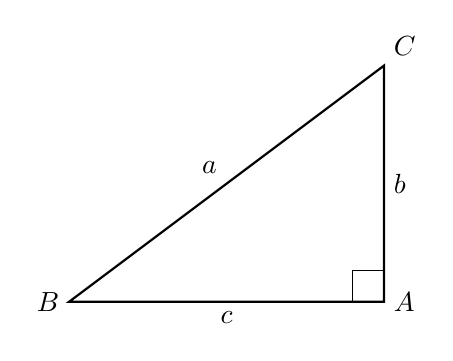
\begin{tikzpicture}
    % Pontos do triângulo
    \coordinate (B) at (0,0);
    \coordinate (A) at (4,0);
    \coordinate (C) at (4,3);

    % Lados do triângulo
    \draw[thick] (B) -- (A) -- (C) -- cycle;

    % Marcação do ângulo reto em A
    \draw (A) ++(-0.4,0) -- ++(0,0.4) -- ++(0.4,0);

    % Nome dos vértices
    \node[right] at (A) {$A$};
    \node[left] at (B) {$B$};
    \node[above right] at (C) {$C$};

    % Lados a, b, c
    \path (B) -- node[above left] {$a$} (C);
    \path (A) -- node[right] {$b$} (C);
    \path (A) -- node[below] {$c$} (B);

    \end{tikzpicture}
    \caption{Triângulo retângulo.}
    \label{fig:triangulo-retangulo}
\end{figure}

    No aspecto vetorial, dados dois vetores $v$ e $w$, perceba que o vetor $v-w=v+(-w)$ pode ser representado como o segmento orientado que une a extremidade de $w$ à extremidade de $v$, conforme ilustrado na Figura~\ref{fig:diferenca-vetores}.

\begin{figure}[ht]
    \centering
    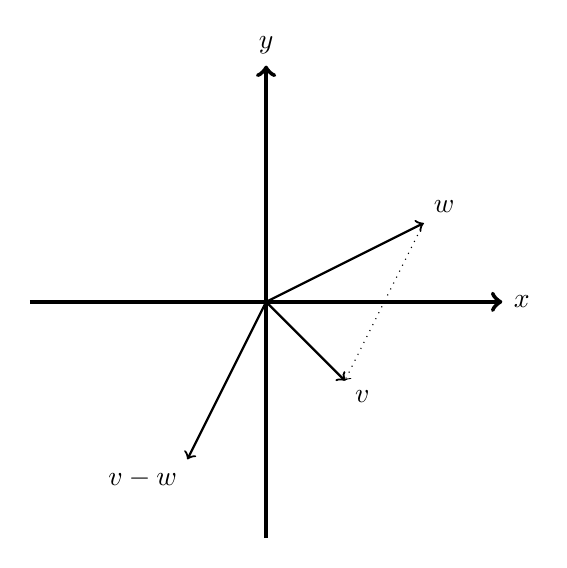
\begin{tikzpicture}
    \draw[->,ultra thick] (-3,0)--(3,0) node[right]{$x$};
    \draw[->,ultra thick] (0,-3)--(0,3) node[above]{$y$};
    % Vetor v
    \draw[->,thick] (0,0) -- (2,1) node[above right]{$w$};
    % Vetor v-w
    \draw[->,thick] (0,0) -- (-1,-2) node[below left]{$v-w$};
    \draw[->,dotted] (2,1) -- (1,-1);
    % Vetor v+w
    \draw[->,thick] (0,0) -- (1,-1) node[below right]{$v$};
    \end{tikzpicture}
    \caption{O vetor $v-w$ como deslocamento da extremidade de $w$ até a extremidade de $v$.}
    \label{fig:diferenca-vetores}
\end{figure}

Motivados pela recíproca do Teorema de Pitágoras, dizemos que dois vetores $v,w\in\mathbb R^n$ são \emph{ortogonais} quando
\[
    \|v-w\|^2=\|v\|^2+\|w\|^2.
\]

\begin{proposition}\index{ortogonalidade!produto escalar}
    Sejam $v, w \in \mathbb R^n$. Então, $v$ e $w$ são ortogonais se, e somente se, $v \cdot w = 0$.
\end{proposition}
\begin{proof}
    Notemos que, no geral:
    \begin{equation*}
        \|v-w\|^2 = (v-w) \cdot (v-w) = v \cdot v - 2v \cdot w + w \cdot w = \|v\|^2 - 2v \cdot w + \|w\|^2.
    \end{equation*}
    Assim, temos que:
    \begin{align*}
        \|v-w\|^2 &= \|v\|^2 + \|w\|^2 \\
        &\iff \|v\|^2 - 2v \cdot w + \|w\|^2 = \|v\|^2 + \|w\|^2 \\
        &\iff -2v \cdot w = 0 \\
        &\iff v \cdot w = 0.
    \end{align*}
\end{proof}

\subsection*{Exercícios}

\begin{exercise}
    Calcule a norma dos seguintes vetores:
    \[
        (3,4),\qquad (1,-2,2),\qquad (2,-1,0,2),\qquad (0,\ldots,0)\in\mathbb R^n.
    \]
\end{exercise}

\begin{exercise}
    Seja $v=(2,-1,2)$.
    Calcule:
    \[
        \|v\|,\qquad \|-v\|,\qquad \|3v\|,\qquad \left\|\frac12v\right\|.
    \]
\end{exercise}

\begin{exercise}
    Determine todos os números reais $\alpha$ tais que, para $v=(1,2,2)$, tenhamos $\|\alpha v\|=9$.
\end{exercise}

\begin{exercise}
    Verifique quais dos seguintes pares de vetores são ortogonais:
    \begin{enumerate}[label=(\alph*)]
        \item $v=(1,2)$ e $w=(2,-1)$;
        \item $v=(1,-1,2)$ e $w=(3,1,-1)$;
        \item $v=(2,0,-1)$ e $w=(1,4,2)$.
    \end{enumerate}
\end{exercise}

\begin{exercise}
    Seja $v=(3,4)$.
    Encontre um vetor $u\in\mathbb R^2$ que tenha a mesma direção e o mesmo sentido de $v$, mas norma igual a $1$.
\end{exercise}

\begin{exercise}
    Seja $v\in\mathbb R^n$ um vetor não nulo.
    Seja
    \[
        u=\frac{1}{\|v\|}v
    \]
    Mostre que $\|u\|=1$.
\end{exercise}

\begin{exercise}
    Sejam $v,w\in\mathbb R^n$.
    Mostre que
    \begin{enumerate}[label=(\alph*)]
        \item $\|-v\|=\|v\|$;
        \item $\|v-w\|=\|w-v\|$;
        \item $\|v+w\|^2=\|v\|^2+2v\cdot w+\|w\|^2$;
        \item $\|v-w\|^2=\|v\|^2-2v\cdot w+\|w\|^2$.
    \end{enumerate}
\end{exercise}

\begin{exercise}
    Sejam $v,w\in\mathbb R^n$.
    Prove que
    \[
        \|v+w\|^2+\|v-w\|^2=2\|v\|^2+2\|w\|^2.
    \]

    Essa igualdade é conhecida como a \emph{identidade do paralelogramo}.
\end{exercise}

\begin{exercise}
    Sejam $v,w\in\mathbb R^n$ vetores ortogonais.
    Mostre que
    \[
        \|v+w\|^2=\|v\|^2+\|w\|^2.
    \]
\end{exercise}

\begin{exercise}
    Use a desigualdade triangular para mostrar que, para todos $v,w\in\mathbb R^n$,
    \[
        \big|\|v\|-\|w\|\big|\leq \|v-w\|.
    \]
\end{exercise}
\section{Distância em \texorpdfstring{$\mathbb R^n$}{Rn}}
A distância euclidiana usual entre dois pontos $p,q\in\mathbb R^n$ é motivada pelo Teorema de Pitágoras:
ela mede o comprimento do vetor deslocamento entre esses dois pontos.

\begin{definition}
    Sejam $p=(p_1,\ldots,p_n)$ e $q=(q_1,\ldots,q_n)$ elementos de $\mathbb R^n$.
    A \emph{distância euclidiana usual}\index{distância euclidiana}\index{métrica euclidiana|see{distância euclidiana}} entre $p$ e $q$ é definida como:
    \begin{equation*}
        d(p, q) = \|p-q\| = \sqrt{(p-q) \cdot (p-q)}=\sqrt{\sum_{i=1}^n (p_i - q_i)^2}.
    \end{equation*}
\end{definition}

Assim, medir a distância entre $p$ e $q$ é medir o comprimento do vetor $p-q$.
Como esse vetor representa um deslocamento entre os dois pontos, a definição acima estende a ideia pitagórica de distância.

No caso $n=1$, identificando $\mathbb R^1$ com $\mathbb R$, se $p,q\in\mathbb R$, então
\[
    d(p,q)=|p-q|.
\]

No caso $n=2$, se $p=(x_1,y_1)$ e $q=(x_2,y_2)$, então
\[
    d(p,q)=\sqrt{(x_1-x_2)^2+(y_1-y_2)^2},
\]
que é exatamente a fórmula da distância no plano cartesiano.

Já no caso $n=3$, se $p=(x_1,y_1,z_1)$ e $q=(x_2,y_2,z_2)$, recuperamos, analogamente, a fórmula usual da distância no espaço tridimensional:
\[
    d(p,q)=\sqrt{(x_1-x_2)^2+(y_1-y_2)^2+(z_1-z_2)^2}.
\]

Para $n\geq 4$, a mesma fórmula será tomada como a extensão natural da distância pitagórica para pontos com $n$ coordenadas.

\begin{example}\label{ex:distanciaRn}
    Se $p=(1,2)$ e $q=(4,6)$, então
    \[
        d(p,q)=\sqrt{(1-4)^2+(2-6)^2}
        =\sqrt{9+16}=5.
    \]
    Geometricamente, estamos calculando o comprimento do vetor
    \[
        p-q=(-3,-4),
    \]
    que representa um deslocamento de $q$ até $p$.
\end{example}

\subimport{distanciaRn}{figura}

As propriedades abaixo formalizam fatos esperados de qualquer boa noção de distância:
a distância nunca é negativa; dois pontos têm distância zero exatamente quando são o mesmo ponto;
a ordem dos pontos não altera a distância entre eles;
e ir diretamente de $p$ até $r$ nunca é mais longo do que ir de $p$ até $q$ e depois de $q$ até $r$.
\begin{proposition}\label{prop:distanciaRn}
    Sejam $p, q, r \in \mathbb R^n$. Então:
    \begin{enumerate}
        \item $d(p, q)\geq 0$, e $d(p, q) = 0$ se, e somente se, $p=q$.
        \item $d(p, q) = d(q, p)$ (simetria);
        \item $d(p, r) \leq d(p, q) + d(q, r)$ (desigualdade triangular).
    \end{enumerate}
\end{proposition}
\begin{proof}
    Vamos verificar cada uma das propriedades.
    \begin{enumerate}
        \item Como $d(p,q)=\|p-q\|$, temos $d(p,q)\geq 0$. Além disso, $d(p, q) = 0$ se, e somente se, $\|p-q\|=0$, o que ocorre se, e somente se, $p-q=0$, ou seja, $p=q$.
        \item Como $q-p=-(p-q)$, temos
        \[
            d(q,p)=\|q-p\|=\|-(p-q)\|=|-1|\|p-q\|=\|p-q\|=d(p,q).
        \]
        \item Como $p-r=(p-q)+(q-r)$, temos:
        \begin{align*}
            d(p, r) &= \|p-r\| = \|(p-q)+(q-r)\| \\
            &\leq \|p-q\| + \|q-r\| = d(p, q) + d(q, r).
        \end{align*}
    \end{enumerate}
\end{proof}

\begin{exercise}
    Calcule as seguintes distâncias:
    \begin{enumerate}[label=(\alph*)]
        \item $d(-3,5)$ em $\mathbb R$;
        \item $d((1,2),(4,6))$ em $\mathbb R^2$;
        \item $d((0,0),(3,4))$ em $\mathbb R^2$;
        \item $d((1,0,-1,2),(3,-1,2,2))$ em $\mathbb R^4$.
    \end{enumerate}
\end{exercise}

\begin{exercise}
    Sejam $p,q,a\in\mathbb R^n$.
    Mostre que
    \[
        d(p+a,q+a)=d(p,q).
    \]
    Interprete geometricamente essa igualdade.
\end{exercise}

\begin{exercise}
    Sejam $p,q\in\mathbb R^n$ e $\alpha\in\mathbb R$.
    Mostre que
    \[
        d(\alpha p,\alpha q)=|\alpha|d(p,q).
    \]
\end{exercise}

\begin{exercise}
    Sejam $p,q,r\in\mathbb R^n$.
    Use a desigualdade triangular para mostrar que
    \[
        d(p,r)-d(q,r)\leq d(p,q).
    \]
    Em seguida, conclua que
    \[
        |d(p,r)-d(q,r)|\leq d(p,q).
    \]
\end{exercise}

\begin{exercise}
    Determine o conjunto de todos os pontos $x\in\mathbb R$ tais que $d(x,3)<2$.
\end{exercise}

